\subsection{Анализ с использованием нейронных сетей}
\label{sec:experiment:neural_engines}

Для сравнения также было решено разработать методику оценки стоимости недвижимости с использованием
нейронных сетей. Задача оценки недвижимости схематично представлена на рисунке~\ref{fig:experiment:neural-scheme}

\begin{figure}[!ht]
  \centering
  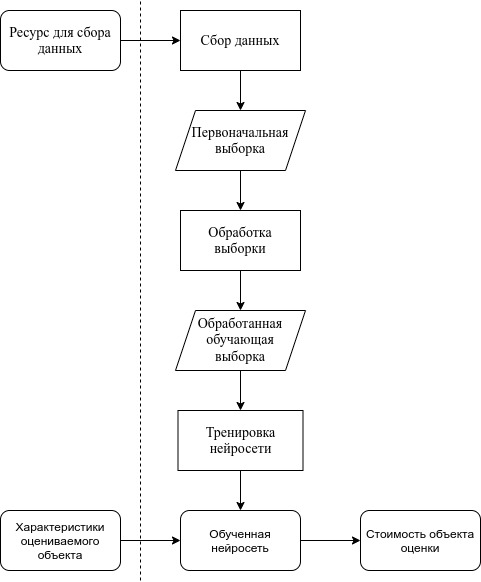
\includegraphics[scale=0.8]{neural-scheme.jpg} 
  \caption{Cхема использования нейронных сетей для оценки стоимости недвижимости}
  \label{fig:experiment:neural-scheme}
\end{figure}

***

Виды нейронных сетей, особенности, отличия

почему выбран именно такой, 

сравнение разных способов на основе других статей

***

Для достижения цели необходимо выбрать факторы, влияющие на	рыночную стоимость объектов недвижимости, подготовить выборку для
обучения нейронной сети. Обучающая выборка построена для проектирования и обучения нейронной сети с учителем,
поскольку такой тип нейронных сетей больше всего подходит для задач, когда имеется большой набор настоящих данных для обучения
алгоритма. Исходя из сравнительного анализа нескольких типов нейронных сетей с учителем, проведенного в статье, было
решено использовать нейронную сеть многослойный персептрон c использованием метода обратного распространения ошибки.
Многослойным персептроном называют нейронную сеть прямого распространения, где входной сигнал распространяется от слоя
к слою в прямом направлении. В общем представлении такая нейронная сеть состоит из:
\begin{itemize}
  \item множества входных узлов, образующих входной слой;
  \item одного или нескольких скрытых слоев вычислительных нейронов;
  \item одного выходного слоя нейронов.
\end{itemize}

Обощенная схема многослойного персептрона показана на рисунке~\ref{fig:experiment:perceptron-scheme}
\begin{figure}[!ht]
  \centering
  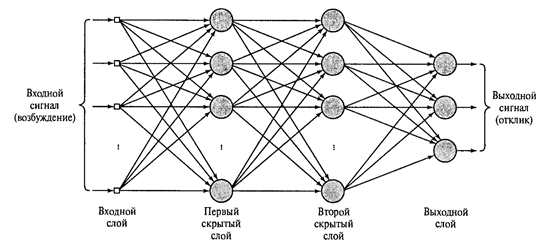
\includegraphics[scale=2]{perceptron.png}
  \caption{Cхема многослойного персептрона}
  \label{fig:experiment:perceptron-scheme}
\end{figure}

Алгоритм обратного распространения ошибки является популярным алгоритмом обучения нейронных сетей с учителем. В основе
идеи алгоритма лежит использование выходной ошибки нейронной сети для вычисления величин коррекции весов нейронов в скрытых слоях
$$
  E = \frac{1}{2}\sum_{i=1}^{k}\left(y-y'\right)^2,\eqno(1)
$$
где: k — число выходных нейронов сети, y — целевое значение, y' — фактическое выходное значение. Алгоритм является
итеративным. На каждой итерации происходит прямой и обратный проходы. На прямом проходе входной вектор распространяется
входов сети к ее выходам, в результате формируется выходной вектор, который соответствует фактическому состоянию весов.
После вычисляется ошибка нейронной сети как разность между фактическим и целевым значениями.
На обратном проходе эта ошибка распространяется от выхода сети к ее входам, и производится коррекция весов нейронов.
Полученные данные дают возможность с достаточной точностью прогнозировать стоимость объектов недвижимости по заданным параметрам.
